% ------------------------------------------------------------------------------
% TYPO3 Version 10.4 - What's New (German Version)
%
% @license	Creative Commons BY-NC-SA 3.0
% @link		https://typo3.org/help/documentation/whats-new/
% @language	German
% ------------------------------------------------------------------------------

\section{Backend User Interface}
\begin{frame}[fragile]
	\frametitle{Backend User Interface}

	\begin{center}\huge{Kapitel 1:}\end{center}
	\begin{center}\huge{\color{typo3darkgrey}\textbf{Backend User Interface}}\end{center}

\end{frame}

% ------------------------------------------------------------------------------
% ...

\begin{frame}[fragile]
	\frametitle{Backend User Interface}
	\framesubtitle{Backend-UI-Anpassungen}

	Leicht veränderte UI der Spalte "Backend-Module".

	\begin{figure}
		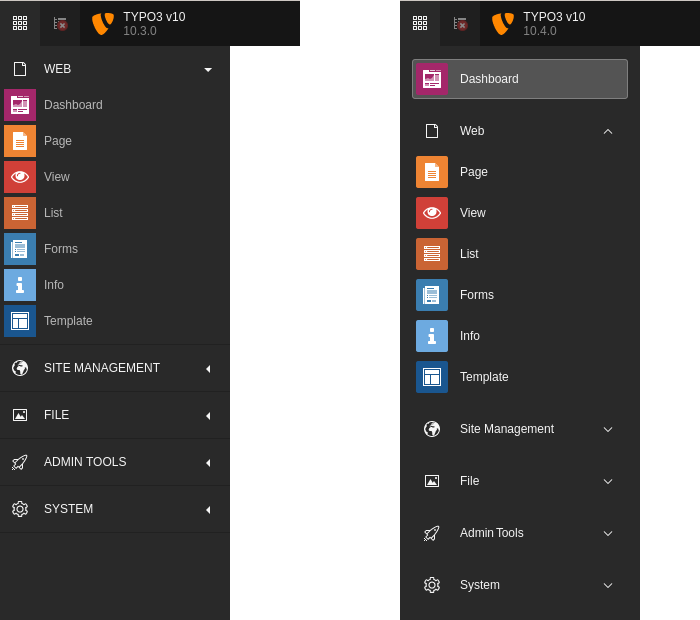
\includegraphics[width=0.5\linewidth]{BackendUserInterface/typo3-backend-ui.png}
	\end{figure}

\end{frame}

% ------------------------------------------------------------------------------
% Feature | 83128 | Content Element Filter

\begin{frame}[fragile]
	\frametitle{Backend User Interface}
	\framesubtitle{Suche nach neuen Inhaltselementen}

	Backend-Benutzer können jetzt im Wizard "Neues Inhaltselement" nach Inhaltselementtypen suchen:

	\begin{figure}
		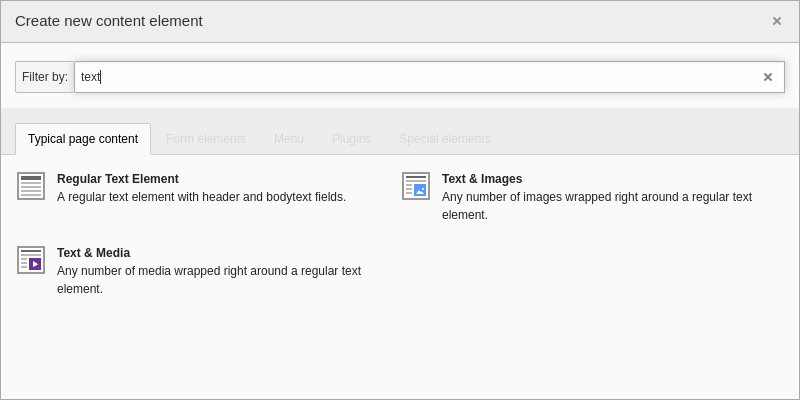
\includegraphics[width=0.6\linewidth]{BackendUserInterface/83128-ContentElementFilter.png}
	\end{figure}

\end{frame}

% ------------------------------------------------------------------------------
% Feature | 89513 | Provide password recovery for backend users

\begin{frame}[fragile]
	\frametitle{Backend User Interface}
	\framesubtitle{Passwort-Wiederherstellung}

	Backend-Benutzer können jetzt eine E-mail zur Passwort-Wiederherstellung anfordern, um ihre Zugangsdaten zurückzusetzen.

	\begin{figure}
		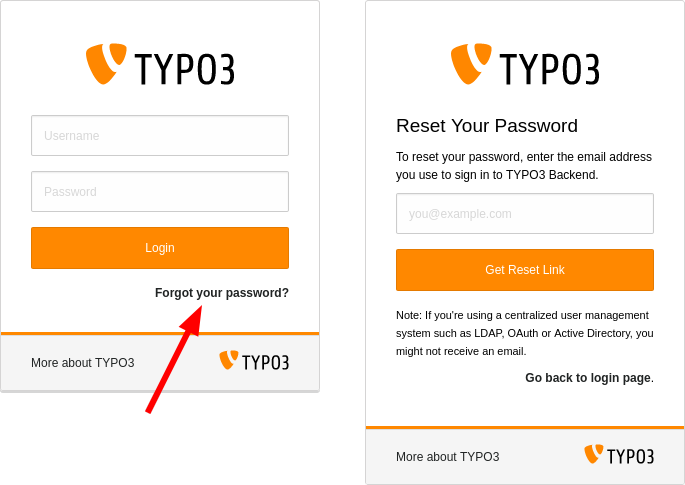
\includegraphics[width=0.6\linewidth]{BackendUserInterface/89513-ProvidePasswordRecoveryForBackendUsers.png}
	\end{figure}

\end{frame}

% ------------------------------------------------------------------------------
